\chapter{考察}
\label{ch:discussion}
\ref{ch:discussion}章ではミリ波分光計を用いて得られた\ref{ch:results}章での結果と、ミリ波分光計以外の外部からのデータの比較とを行う。
\ref{sec:comparison_sofie}節では、ノルウェー・トロムソにおける解析結果(\ref{sec:results_tromsoe}節)に対し、SOFIE(Solar Occultation for Ice Experiment。詳細は付録~\ref{app:sofie})によって観測された\ce{NO}密度の高度プロファイルデータを用いて比較を行う。
\ref{sec:comparison_eep}節では、観測された\ce{NO}柱密度の変動に対するEPPの影響を調べるため、高エネルギー電子の降り込み(EEP: Energetic Electron Precipitation)との比較を行う。


\section{SOFIEの観測データから導出されたNO柱密度との比較}
\label{sec:comparison_sofie}
まずは、ミリ波分光計を用いた\ce{NO}の観測データの妥当性を検証するため、SOFIEによって観測された\ce{NO}の高度プロファイルデータと比較する。
SOFIEのデータは、トロムソで\ce{NO}柱密度を導出した期間と同じ期間にトロムソ付近の緯度(およそ$65 - 80$\textdegree Nの範囲)で観測された高度ごとの\ce{NO}密度のデータを用いた。
なお、昭和基地においては、ミリ波分光計のデータ解析を行った期間のSOFIE観測データが\today 時点で公開されていないため、比較を行っていない。\par
% 仮綴じでは today = 2024-01-26となっている。

図~\ref{fig:sofie_mmcd}に、ミリ波分光計によって得られた\ce{NO}柱密度の時間変化と、SOFIEによって得られた\ce{NO}柱密度の時間変化と、SOFIEによって得られた\ce{NO}柱密度の高度プロファイルの時間変化を示す。
\begin{figure}[htbp]
    \centering
    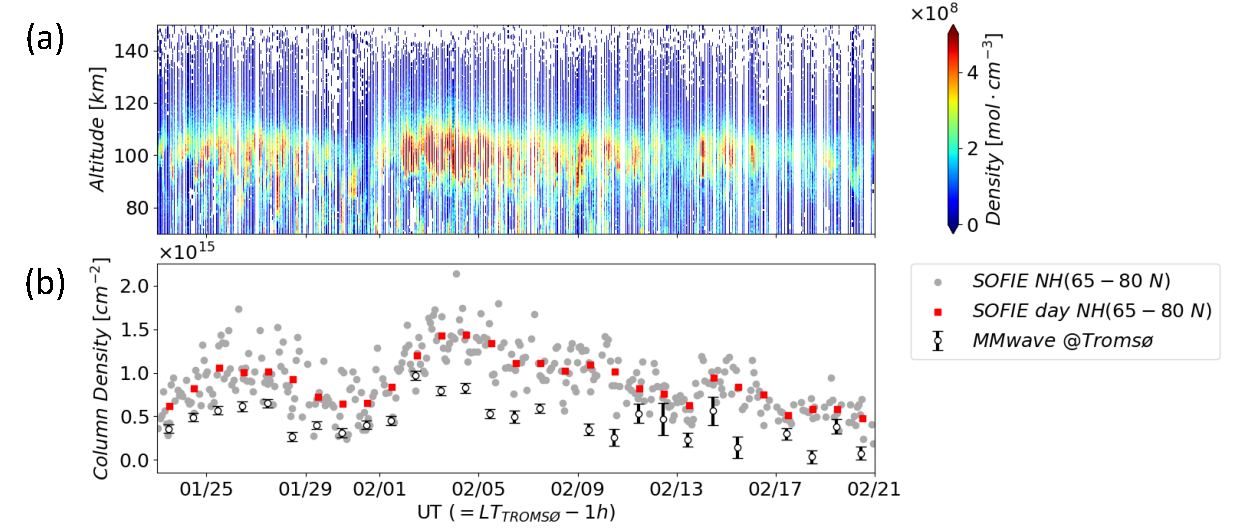
\includegraphics[width=\linewidth]{master_thesis_contents/master_thesis_fig/sofie_mmcd.pdf}
    \caption{(a)SOFIEの\ce{NO}密度の高度プロファイルデータおよび(b)ミリ波分光計を用いて導出したトロムソの柱密度とSOFIEの\ce{NO}密度の高度プロファイルデータから導出した柱密度の比較(エラーバー付きのプロットがミリ波データから導出した柱密度、グレーの丸形プロットがSOFIEの\ce{NO}密度の高度プロファイルデータから導出した柱密度、赤色の四角プロットが1日平均したSOFIEの柱密度)}
    \label{fig:sofie_mmcd}
\end{figure}
ミリ波分光計によって柱密度の増加が確認された2つの期間(2019年1月23日〜2019年1月27日と2019年2月1日〜2019年2月4日)では、SOFIEの高度プロファイルデータでも高度$100\ \mathrm{km}$付近において\ce{NO}の密度の増加が確認できた(図~\ref{fig:sofie_mmcd}(a))。\par

また、ミリ波分光計を用いて導出した柱密度と直接比較を行うため、SOFIEの\ce{NO}密度の高度プロファイルデータを高度方向に足し合わせて、柱密度を導出した(図~\ref{fig:sofie_mmcd}(b)のグレーの丸形プロット)。
これをさらに1日平均した値をが図~\ref{fig:sofie_mmcd}(b)の赤い四角プロットである。
これらを比較した結果、ミリ波分光計による柱密度の時間変動の傾向が、SOFIEから導出した柱密度とよく一致していることが分かった。
しかし、全体的にSOFIEから導出した柱密度の方が、ミリ波分光計による柱密度と比べて全体的に値が大きいことが分かった。\par

柱密度を導出する際に用いた式(\ref{sec:derive_columndensity}節の式\eqref{eq:derive_columndensity})を見ると、第1項$\mathrm{A}$と第2項$T_{\mathrm{atm}}$は観測条件によらない定数であり、第3項$\int T_{\mathrm{NO}}d\nu$のみが変数となるため、SOFIEから導出した柱密度とミリ波分光計による柱密度には定常倍のオフセットがあると仮定して二値の比較を行った。
\begin{figure}[htbp]
    \centering
    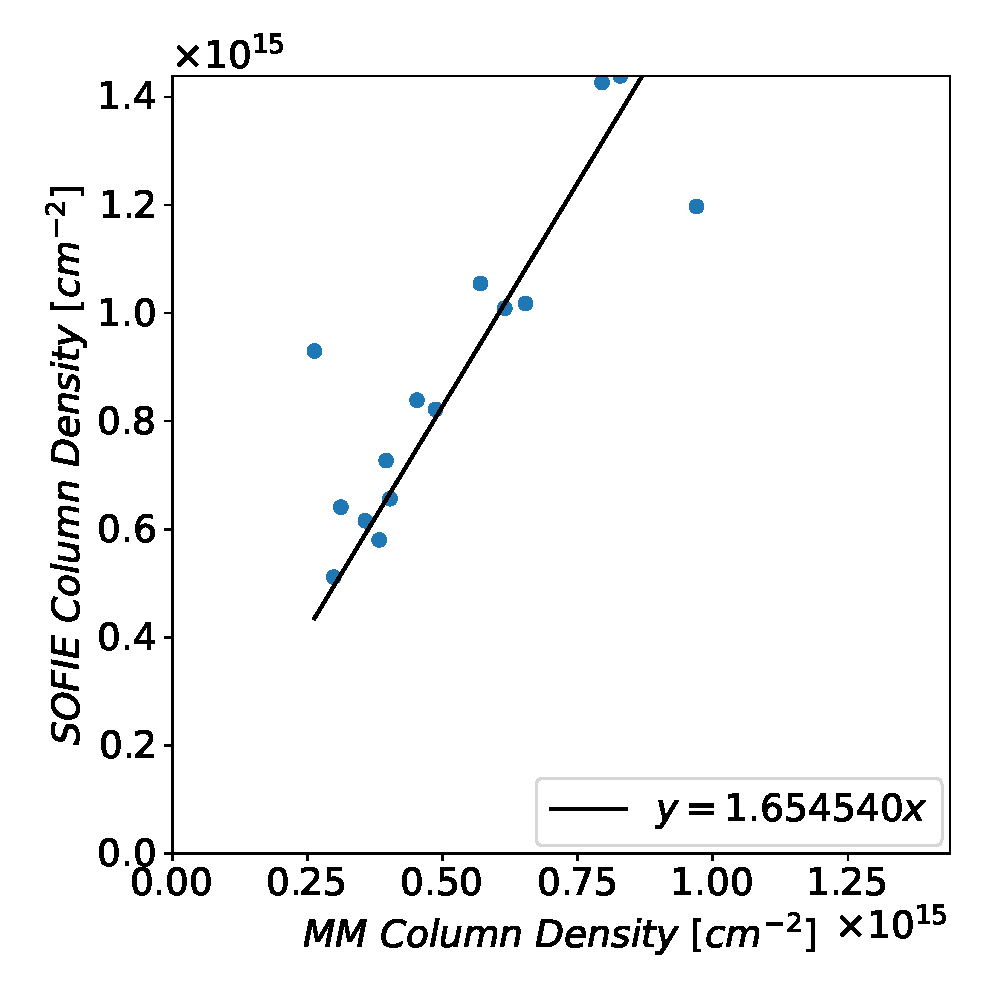
\includegraphics[scale=0.5]{master_thesis_contents/master_thesis_fig/sofie_mmcd_sofiecd_corr.pdf}
    \caption{ミリ波分光計から求めた柱密度(横軸)とSOFIEデータから求めた柱密度の1日平均値(縦軸)との散布図(青色のプロット。黒線は一次近似による直線を示し、右下はその式を表している)}
    \label{fig:sofie_mmcd_sofiecd_corr}
\end{figure}
ミリ波分光計から求めた柱密度とSOFIEデータから求めた柱密度の1日平均値について散布図を作成した結果を図~\ref{fig:sofie_mmcd_sofiecd_corr}に示す。
ただし、スクリーニングされた期間(2019年2月5日〜2019年2月16日)と、検知限界($2\times 10^{14}\ \mathrm{cm^{-2}}$)を下回るデータは含めていない。
また、近似直線は切片を0に固定している(図~\ref{fig:sofie_mmcd_sofiecd_corr}の黒線。近似直線の式は図の右下に示す)。
この結果より、SOFIEによる\ce{NO}柱密度はミリ波分光計による柱密度のおよそ1.65倍の大きさであることが分かった。
この原因のひとつとして、ミリ波分光計で柱密度を導出する際に仮定した大気温度(\ref{sec:derive_columndensity}節の式\eqref{eq:derive_columndensity}の第2項$T_{\mathrm{atm}}$)の値が妥当ではない可能性が考えられる。\par
% コメント:「仮定した大気温度」SOFIEのほうは、何ケルビンか仮定されているのか。
そこで、NRLMSIS 2.0\footnote{\url{https://ccmc.gsfc.nasa.gov/models/NRLMSIS~00/}}を用いて、大気温度の妥当な値を調べた。
これを用いて、2019年1月25日と2月2日(ミリ波分光計を用いて導出した\ce{NO}の柱密度の時間変動のピーク)における高度$100\ \mathrm{km}$付近(SOFIEの\ce{NO}の密度の高度プロファイルデータにおける、ピークがある高度)の大気温度を調べたところ、およそ$180-250\ \mathrm{K}$の範囲であった。
仮に大気温度を$250\ \mathrm{K}$に仮定し直すと、ミリ波分光計を用いて導出した\ce{NO}の柱密度は1.25倍されるが、これだけではSOFIEで導出した\ce{NO}の柱密度との値の差を説明することはできない。
また、大気温度を高度に依存せず一様と仮定していることも原因として考えられるため、大気温度を高度ごとに設定することも考慮に入れる必要がある。
繰り返しになるが、解析期間内において北半球の高緯度領域(およそ$65 - 80$\textdegree Nの範囲)を全体的に観測を行うSOFIEと、トロムソで一定点観測を行うミリ波分光計では、観測の対象領域に違いがある。
これに関しては、モデル計算の結果とミリ波分光計による観測結果と比較することで解決できる可能性が考えられる。


\section{高エネルギー電子の降り込みとの比較}
\label{sec:comparison_eep}
次に、ミリ波分光計の観測から見出された\ce{NO}柱密度変動に対するEPPの影響を調べるため、高エネルギー電子の降り込みとの比較を行った。
比較対象として以下の3種類のデータを用い、各節に分けて比較結果を述べる。
\begin{itemize}
    \item Dst指数(\ref{ssec:comparison_dst}節)
    \item POES/MetOp衛星で観測された電子フラックスデータ(\ref{ssec:comparison_poes}節)
    \item NASAが提供しているOMNI Data Set(\ref{ssec:comparison_omni}節)
\end{itemize} \par
Dst指数、POES/MetOp、OMNI Data Setの詳細はそれぞれ付録~\ref{app:dst}、付録~\ref{app:poes}、付録~\ref{app:omni}にて紹介している。


\subsection{Dst指数との比較}
\label{ssec:comparison_dst}
まずは、Dst指数との比較を行った。
Dst指数とは、地磁気擾乱の大きさを表す指数であり、地磁気擾乱が起きる際に発生する、地球を取り巻く環状の電流(Ring Current)がどの程度地球磁場を打ち消すかを表したものである(詳細は付録~\ref{app:dst})。
Dst指数のデータは、地磁気世界資料センター京都(WDC for Geomagnetism, Kyoto)\footnote{\url{https://wdc.kugi.kyoto-u.ac.jp/wdc/Sec3.html}}より調べた。\par
トロムソにおける柱密度との比較結果を図~\ref{fig:dst_mmcd_tromsoe}、昭和基地における柱密度との比較結果を図~\ref{fig:dst_mmcd_syowa}に示す。
\begin{figure}[htbp]
    \centering
    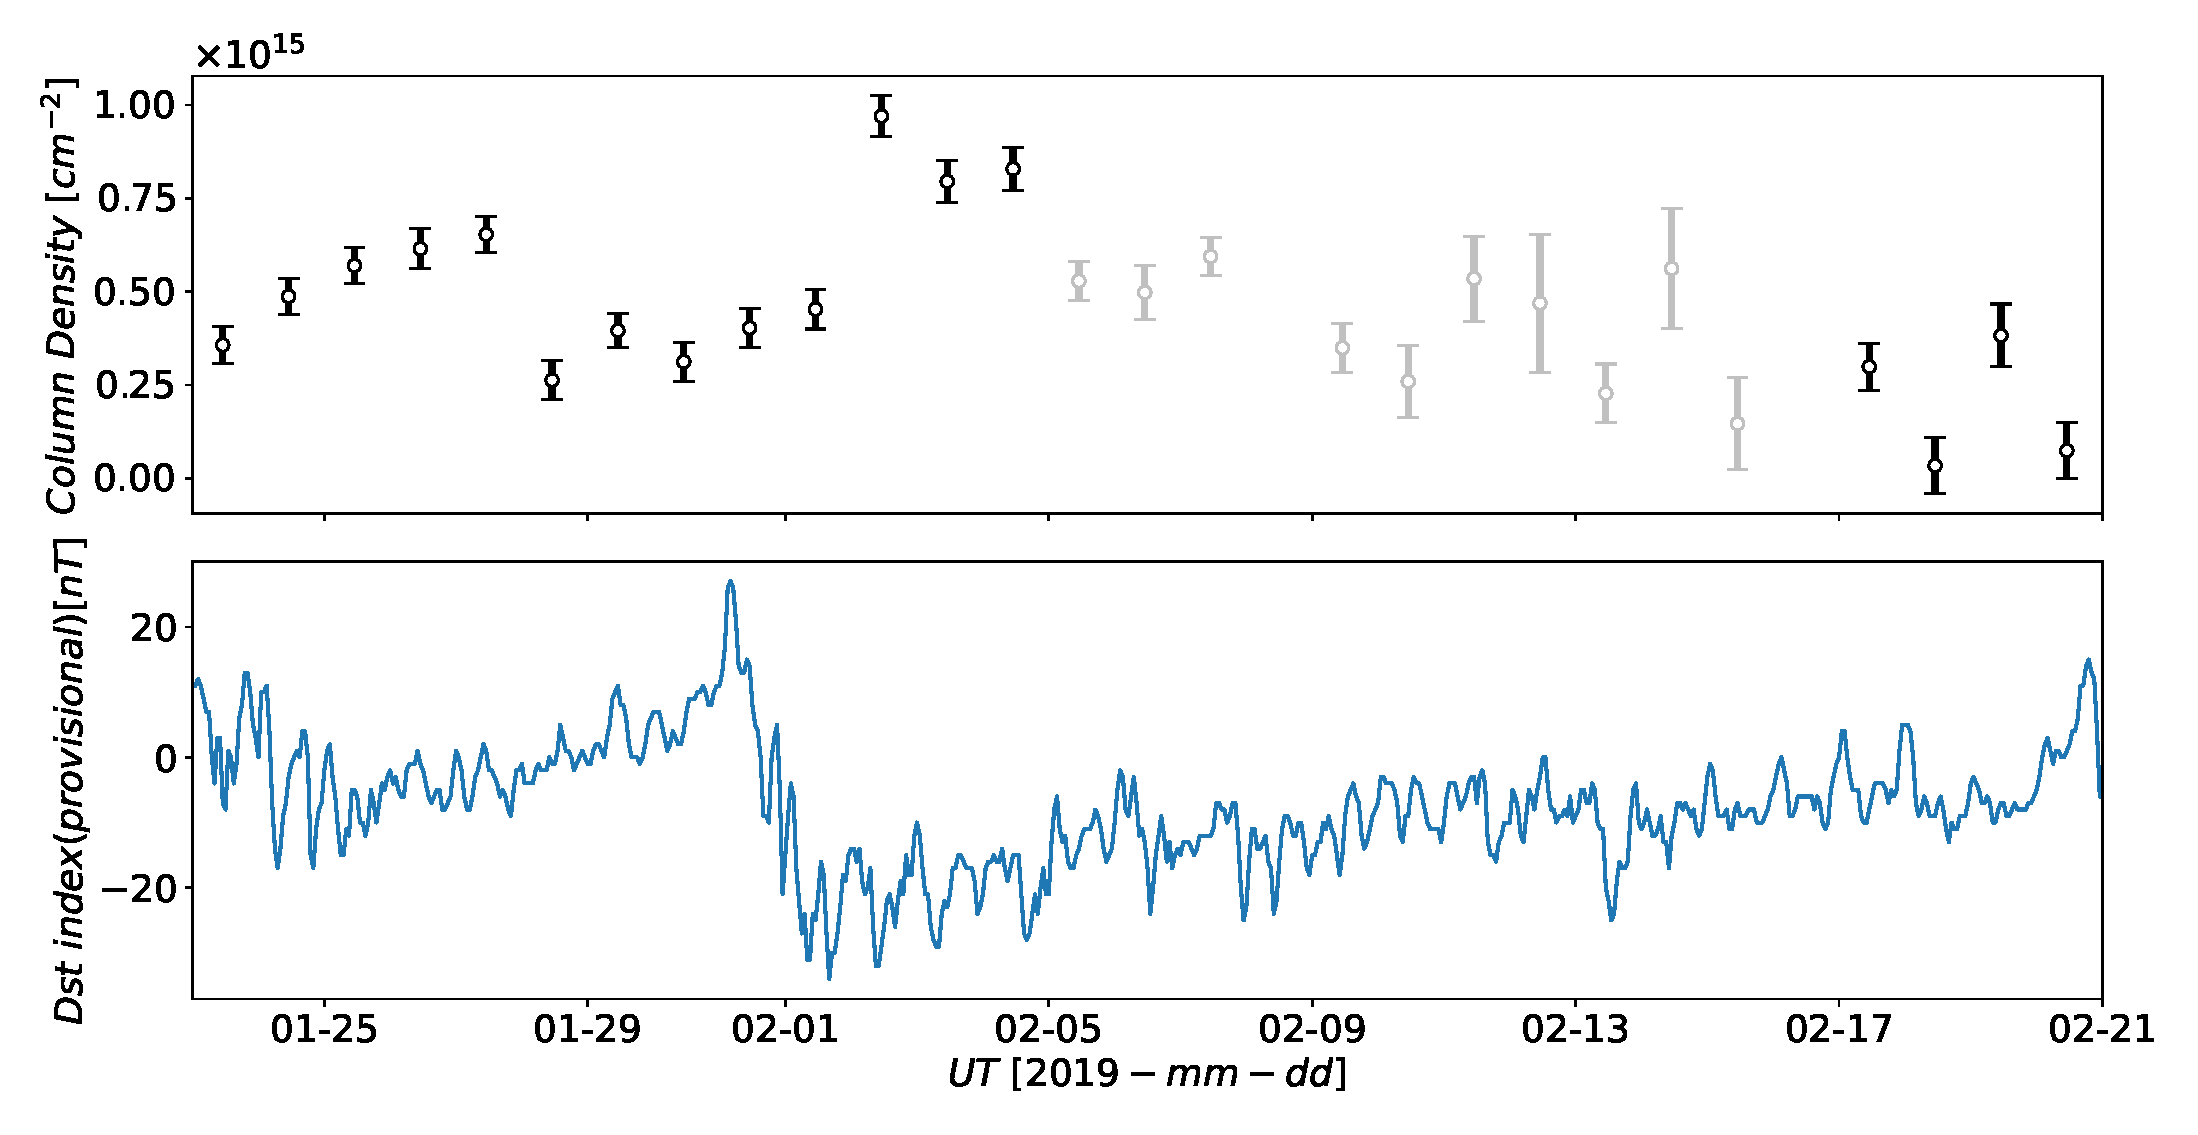
\includegraphics[width=\linewidth]{master_thesis_contents/master_thesis_fig/dst_tromsoe_mmcd.pdf}
    \caption{トロムソにおける柱密度(1段目。図~\ref{fig:column_density_spectr6_syowa}と同様)とDst指数 暫定値(2段目)との比較}
    \label{fig:dst_mmcd_tromsoe}
\end{figure}
\begin{figure}[htbp]
    \centering
    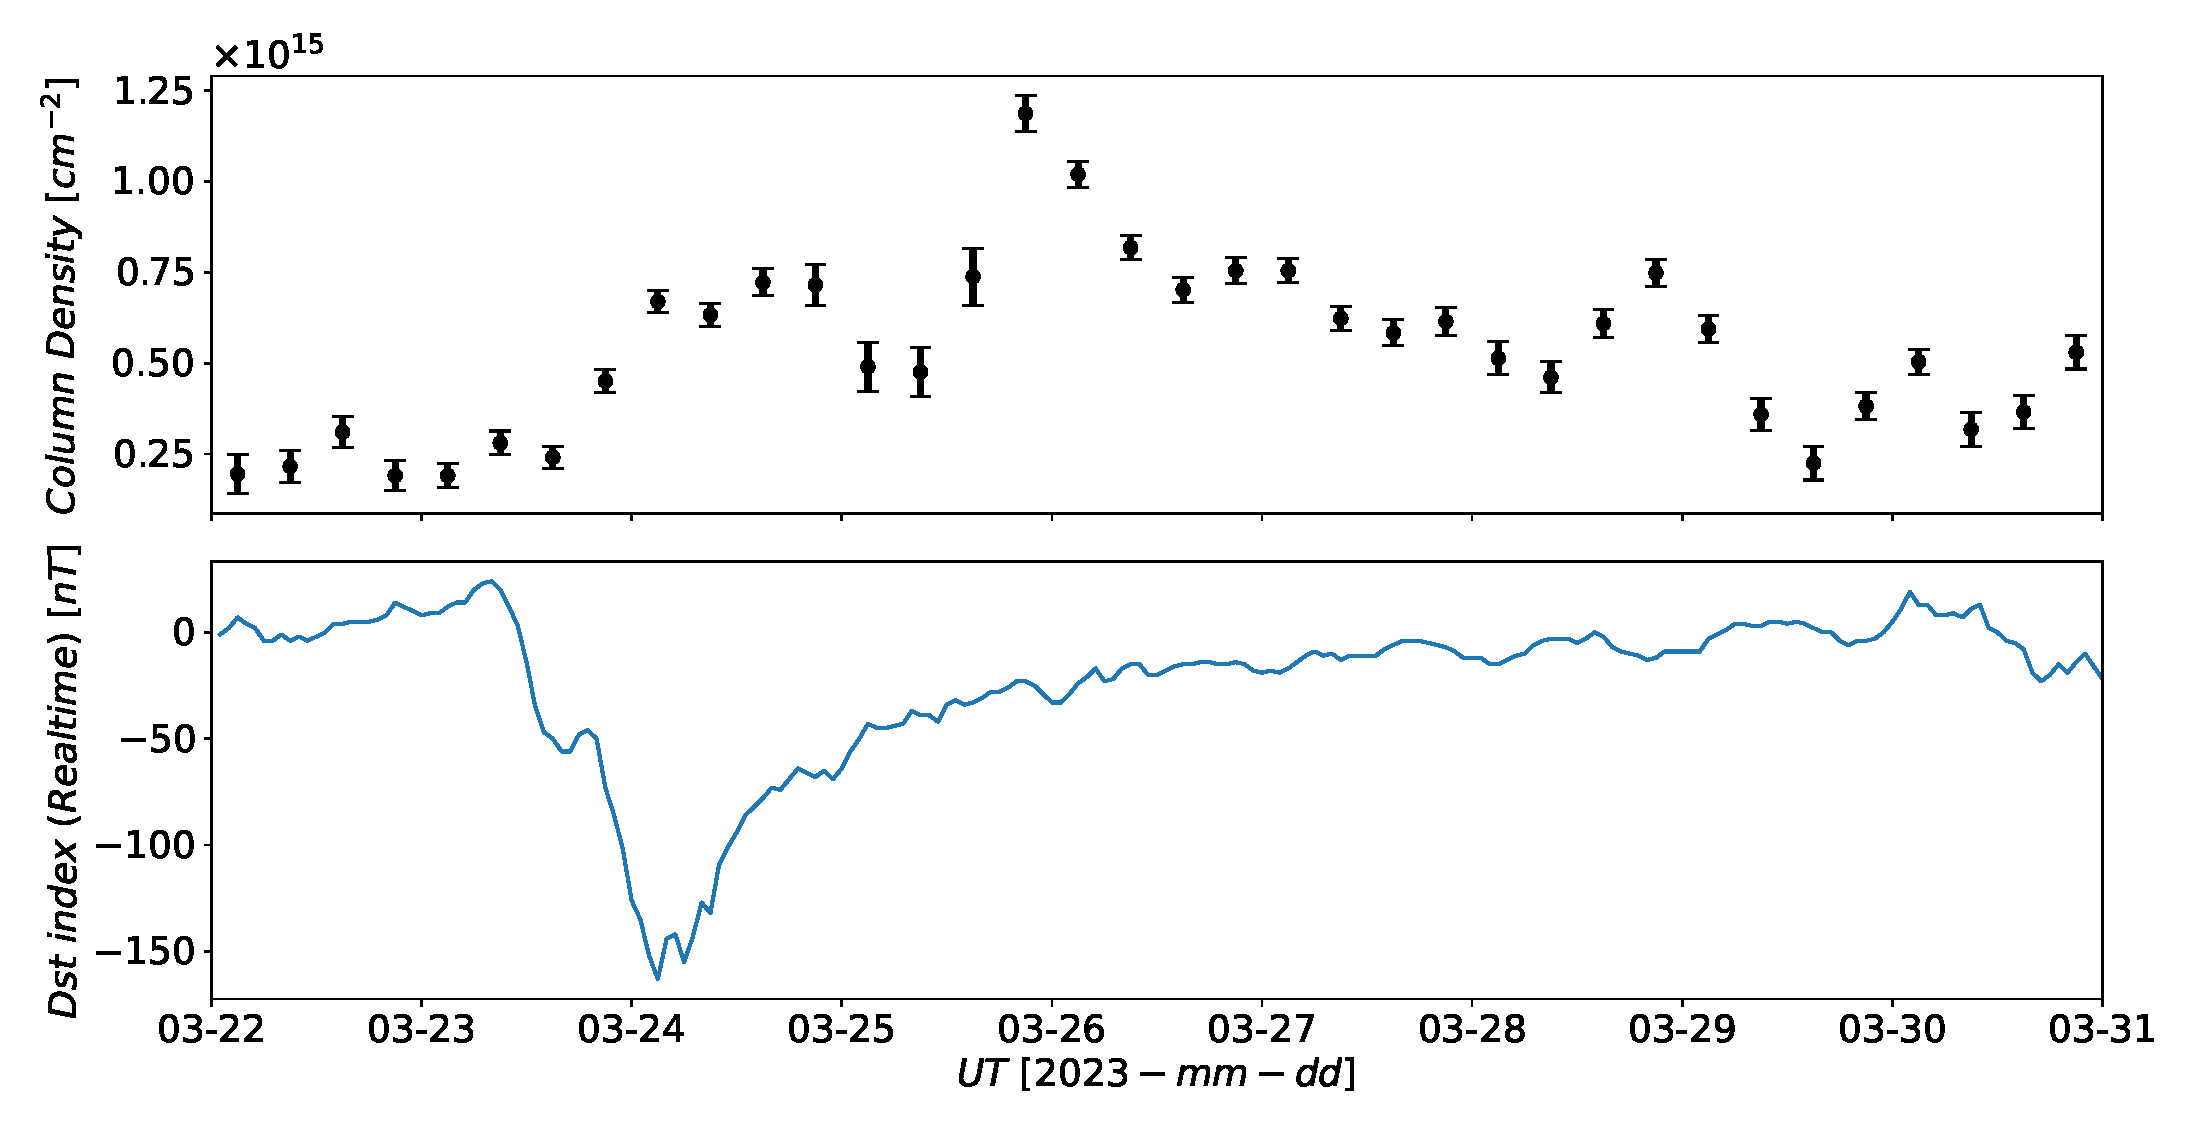
\includegraphics[width=\linewidth]{master_thesis_contents/master_thesis_fig/column_density_spectr6_dst_syowa.pdf}
    \caption{昭和基地における柱密度(1段目。図~\ref{fig:column_density_spectr6_syowa}と同様)とDst指数 速報値(2段目)との比較}
    \label{fig:dst_mmcd_syowa}
\end{figure}
\ce{NO}の柱密度の増加が確認できた期間に対応して、Dst指数の急激な減少がみられた。
とくに、トロムソにおいては急激な\ce{NO}の柱密度の増加があった2019年2月1日〜2019年2月4日、昭和基地においては2023年3月24日の未明前後における\ce{NO}の柱密度の増加によく対応している。
また、比較的小規模ではあるが、トロムソにおいては2019年1月23日〜2019年1月27日においても、Dst指数の減少が確認された。
この結果より地磁気擾乱によって加速されて極域に降り込んだ電子により、\ce{NO}が増加した可能性が考えられる。
しかし、それ以外で\ce{NO}の柱密度の増加が確認できた期間については、Dst指数の減少は確認できなかった。


\subsection{POES/MetOp衛星の電子フラックスデータとの比較}
\label{ssec:comparison_poes}
次に、どのようなエネルギーレンジの電子の降り込みが影響しているかを調べるため、POES/MetOp衛星の電子フラックスデータを用いた比較を行った。
ミリ波分光計の観測場所周辺に降り込む電子のフラックスのみを調べるため、用いるデータについては事前に絞り込みを行った(詳細は付録~\ref{app:poes})。
この比較結果を見ると、トロムソと昭和基地における比較結果をそれぞれ図~\ref{fig:poes_mmcd_tromsoe}、図~\ref{fig:poes_mmcd_syowa}に示す。
電子フラックスデータは電子がもつエネルギーについて、4つの範囲($>40\ \mathrm{keV}$, $>130\ \mathrm{keV}$, $>287\ \mathrm{keV}$, $>612\ \mathrm{keV}$)に分けて表してある。
\begin{figure}[htbp]
    \centering
    \begin{minipage}{\linewidth}
        \centering
        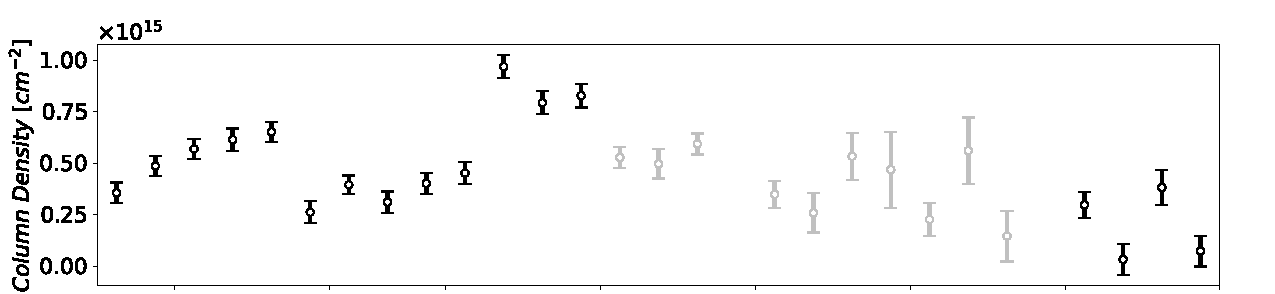
\includegraphics[width=\linewidth]{master_thesis_contents/master_thesis_fig/avg_ColumnDensity_tromsoe_trim.pdf}
    \end{minipage}
    \begin{minipage}{\linewidth}
        \centering
        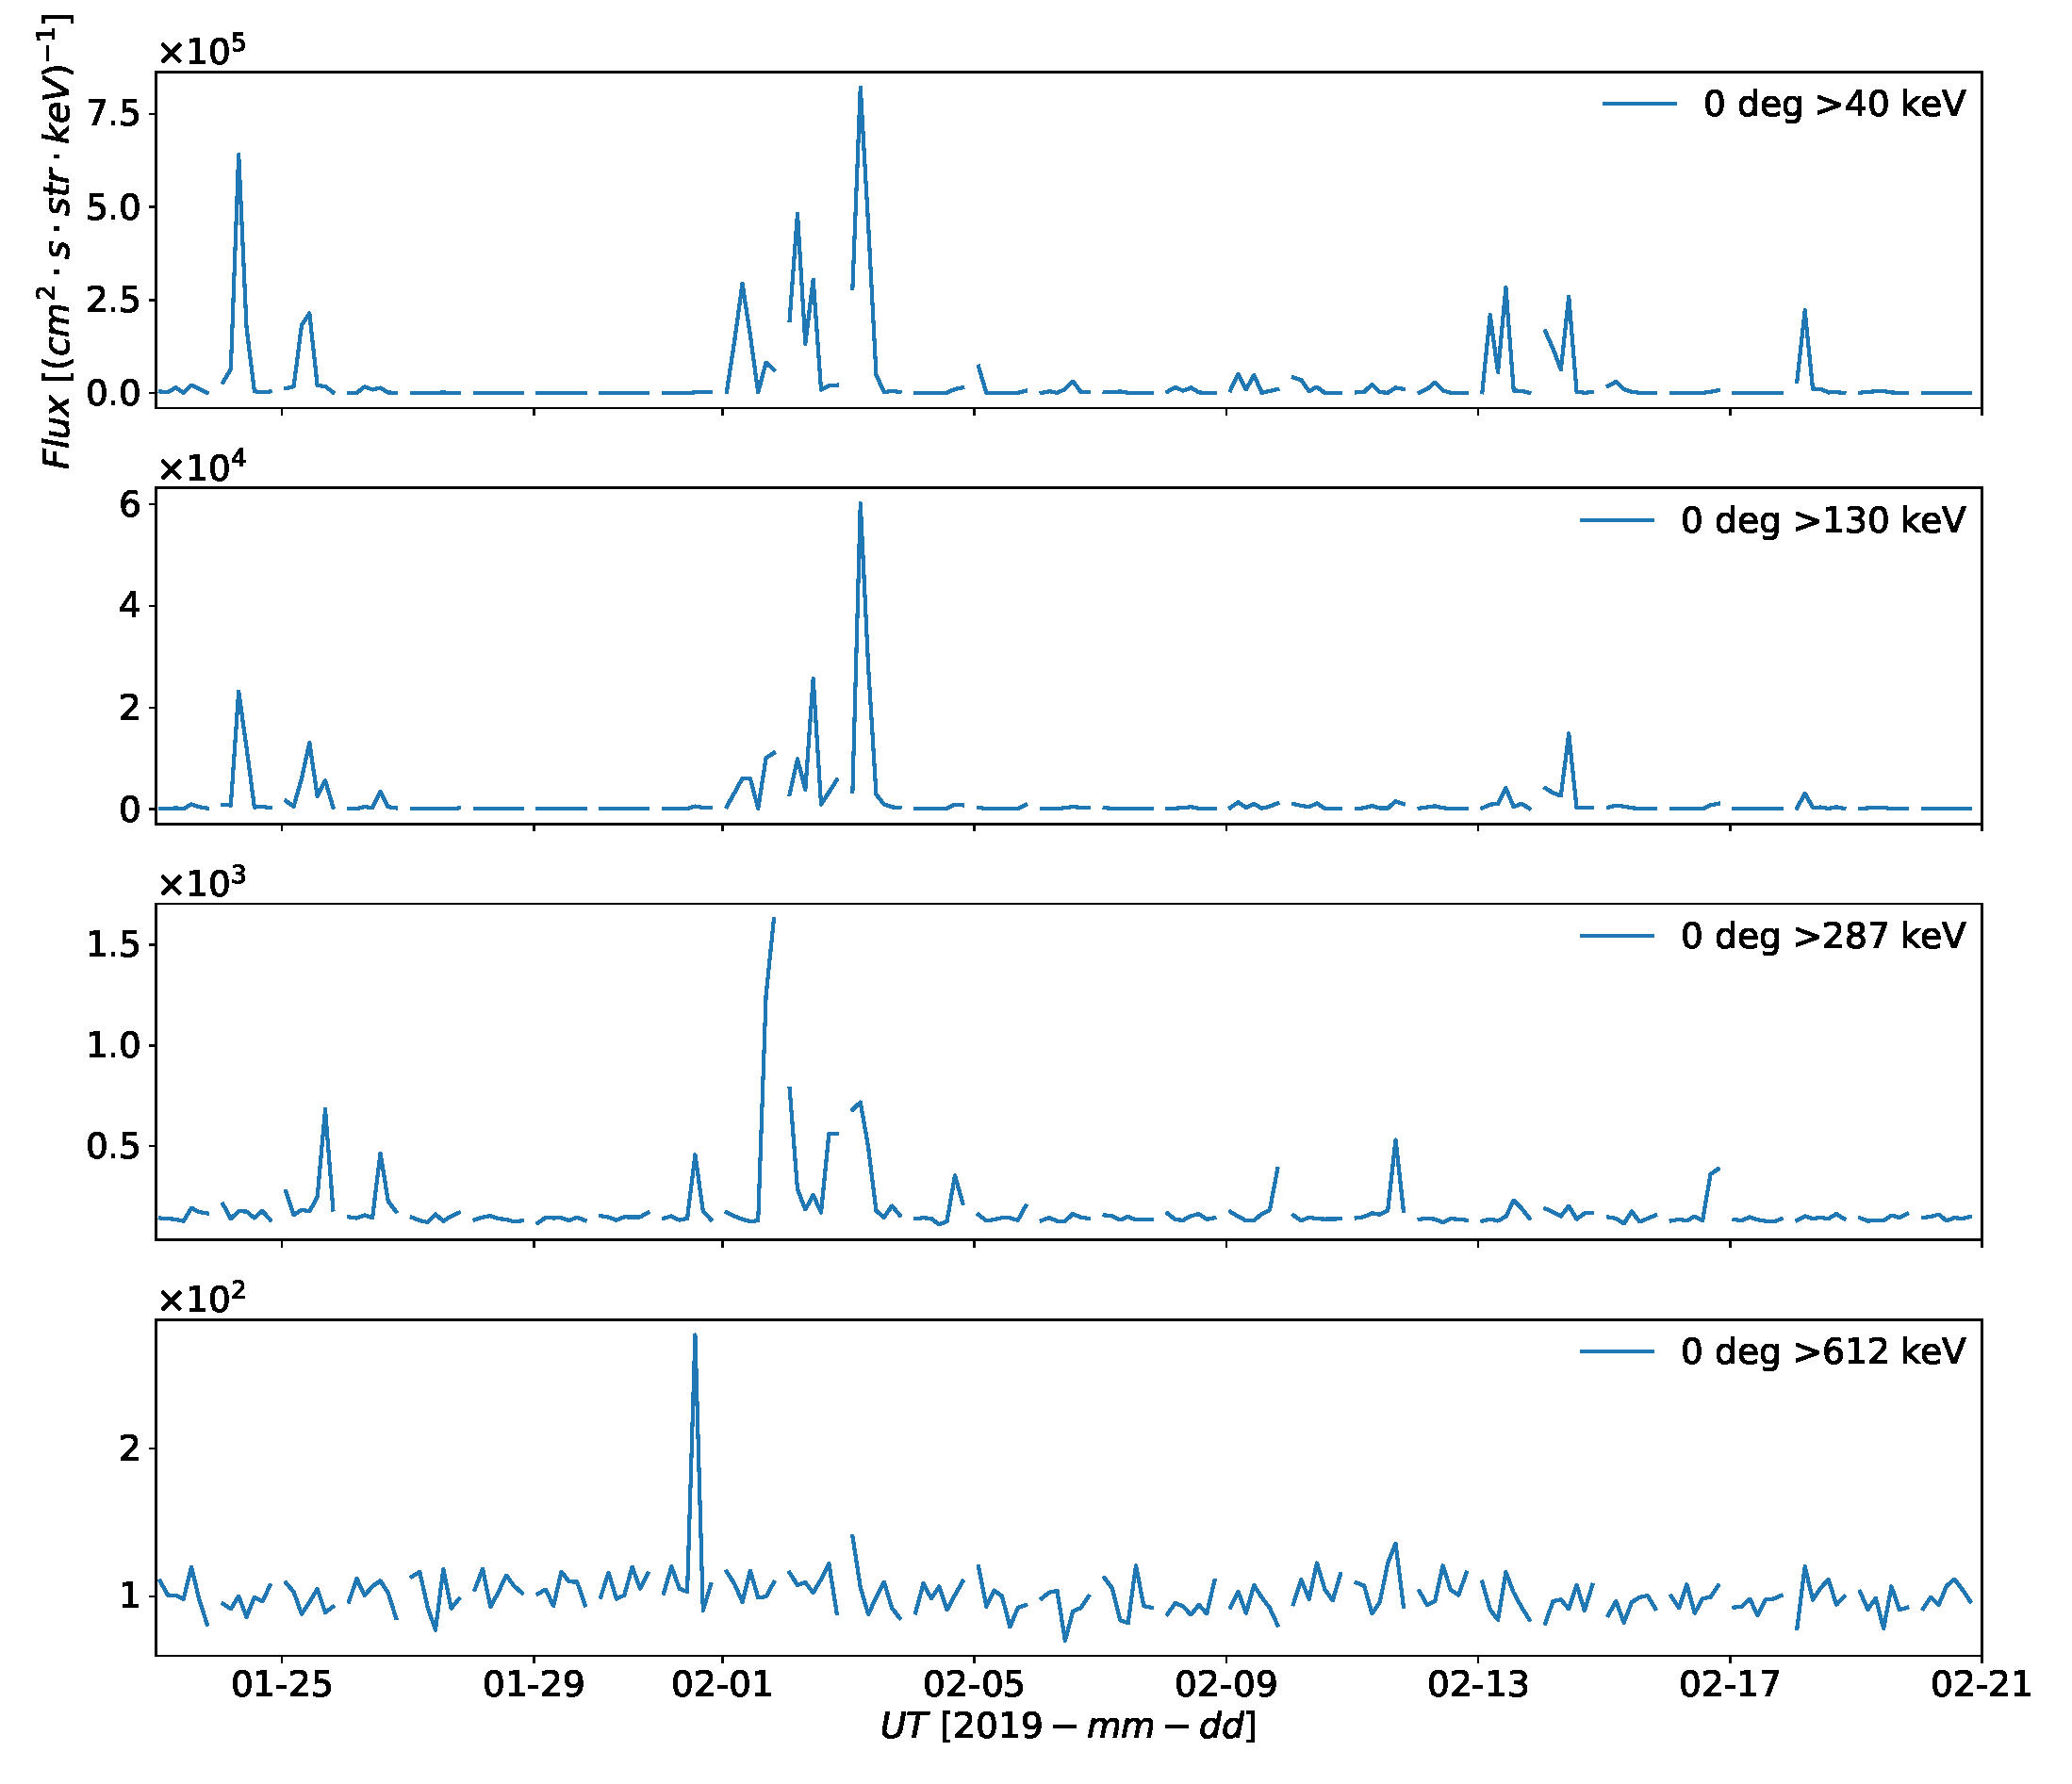
\includegraphics[width=\linewidth]{master_thesis_contents/master_thesis_fig/poes_tromsoe_0deg.pdf}
    \end{minipage}
    \caption{トロムソにおける柱密度(1段目。図~\ref{fig:avg_ColumnDensity_tromsoe}と同様)と電子フラックスデータ(2-5段目)との比較}
    \label{fig:poes_mmcd_tromsoe}
\end{figure}
\begin{figure}[htbp]
    \centering
    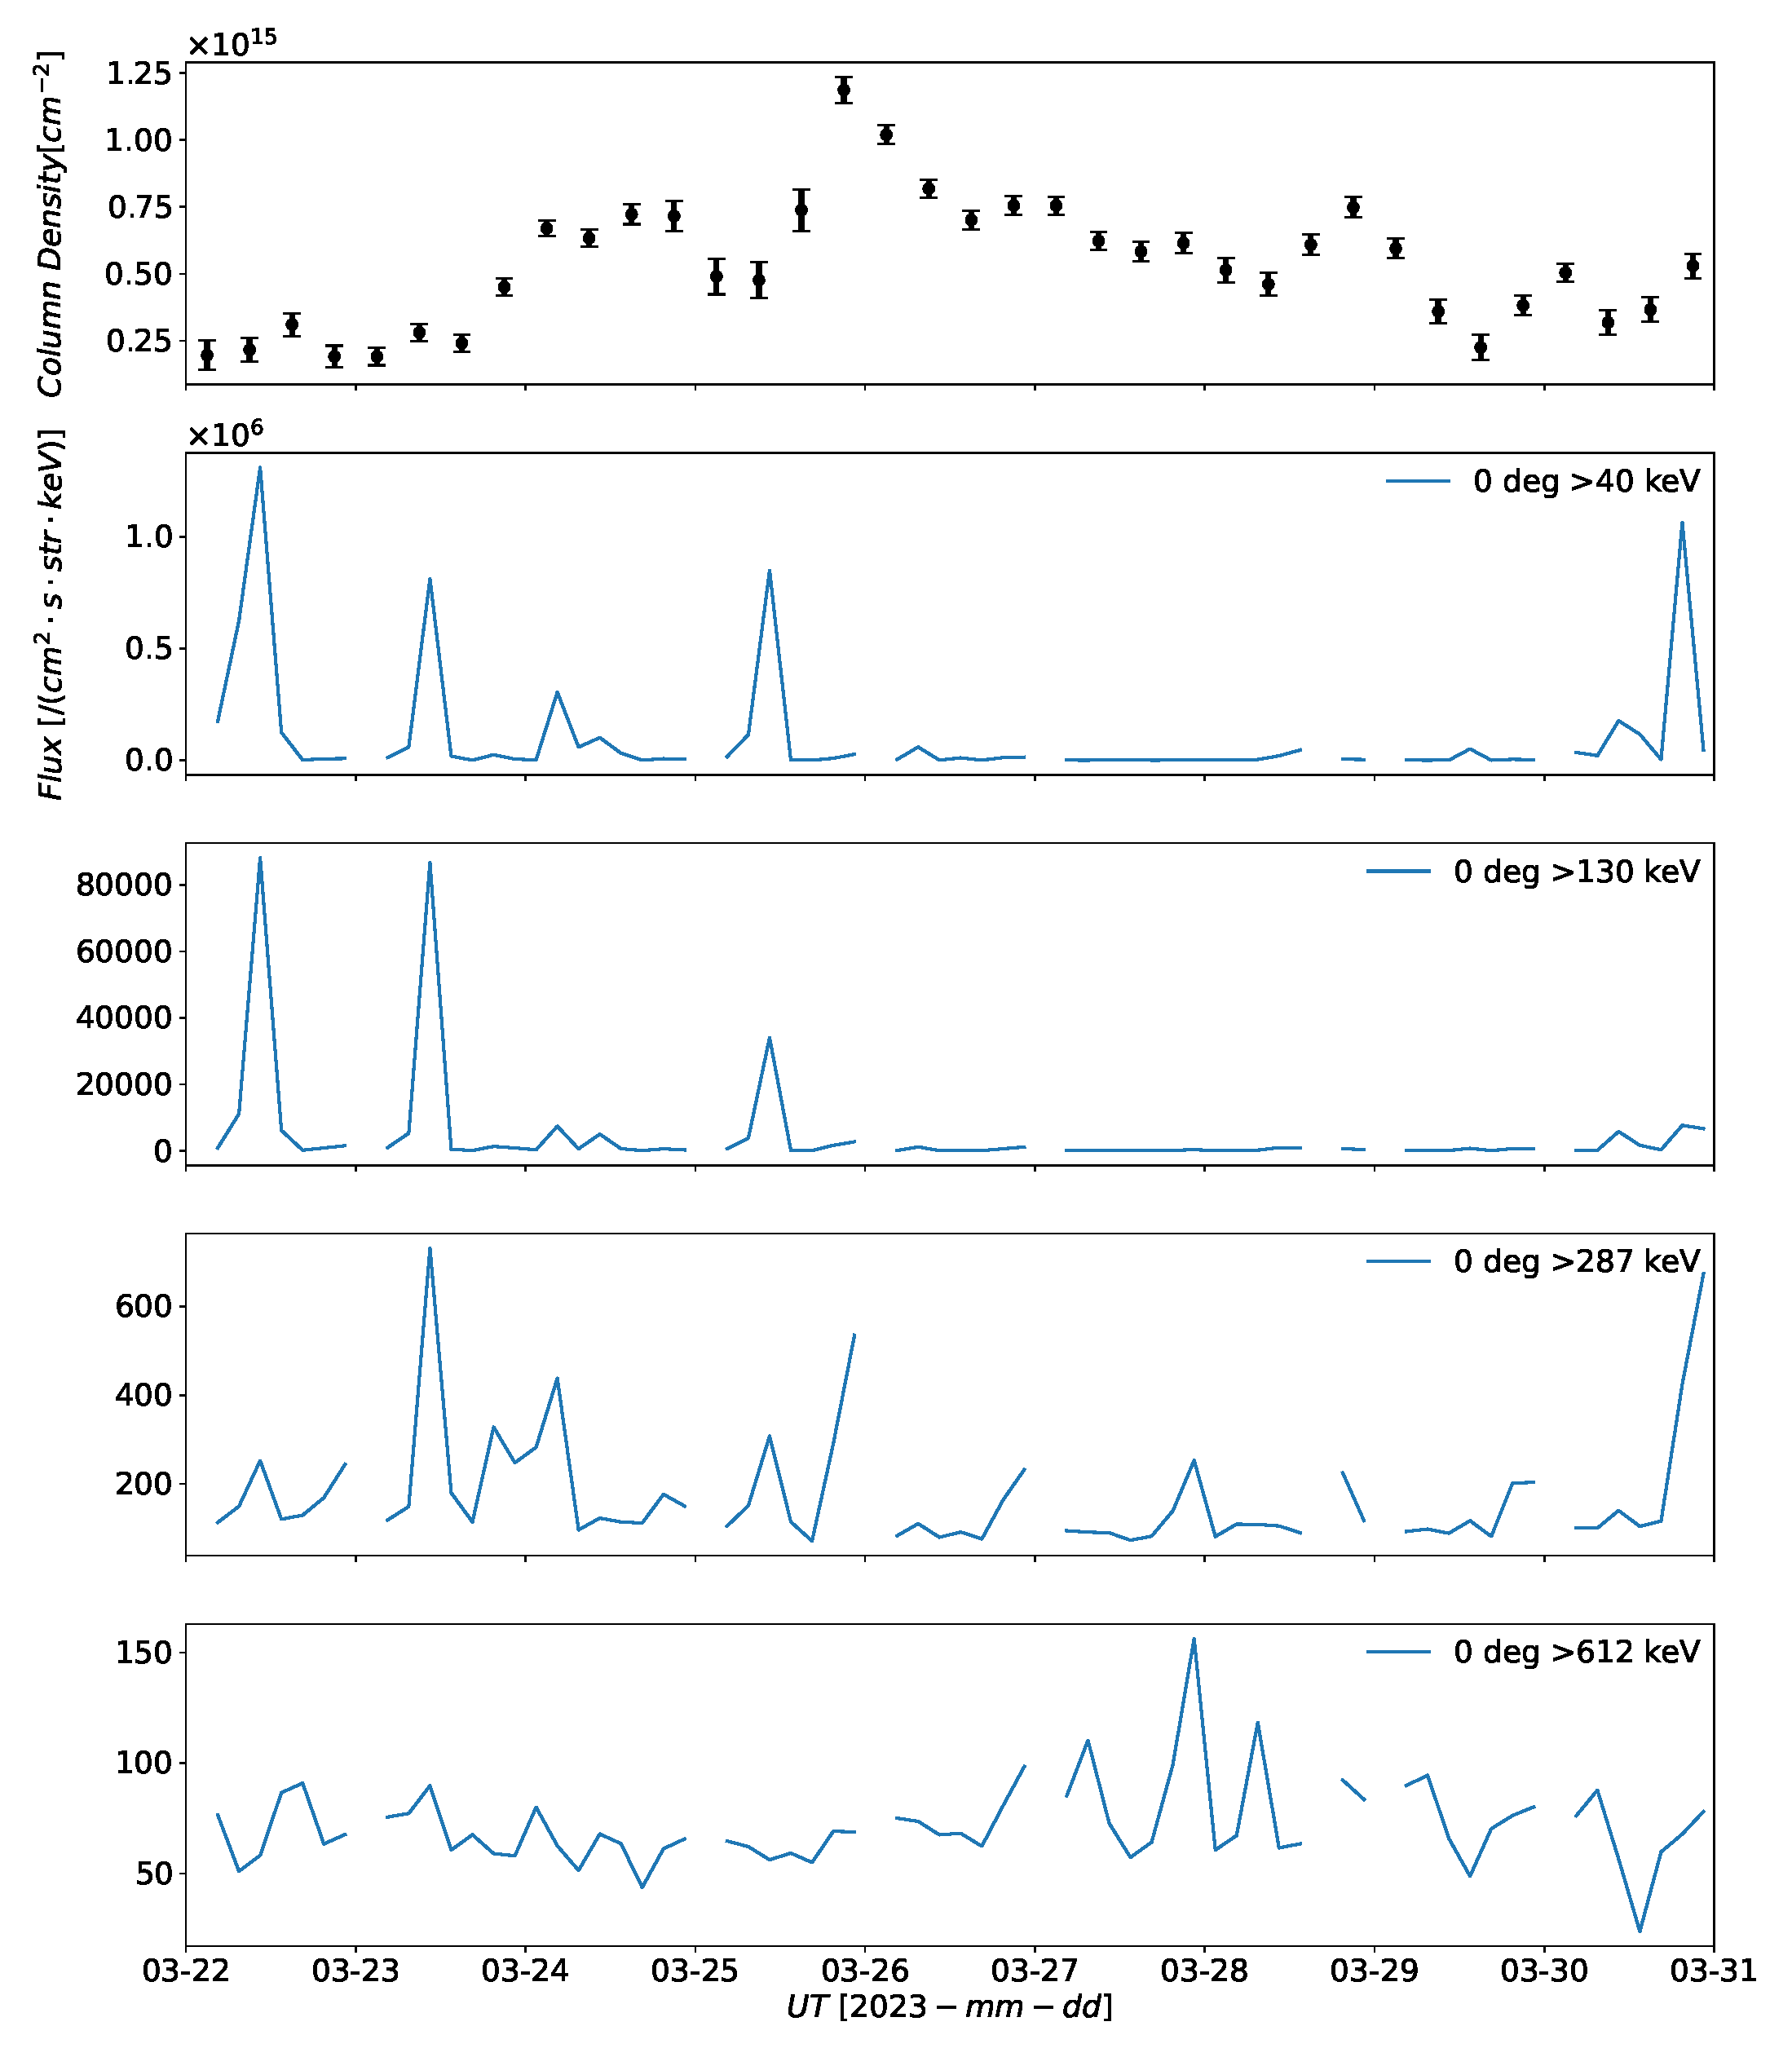
\includegraphics[width=\linewidth]{master_thesis_contents/master_thesis_fig/column_density_spectr6_poes0deg_syowa.pdf}
    \caption{昭和基地における柱密度(1段目。図~\ref{fig:column_density_spectr6_syowa}と同様)と電子フラックスデータ(2-5段目)との比較}
    \label{fig:poes_mmcd_syowa}
\end{figure} \par

トロムソと昭和基地どちらにおいても、すべての柱密度の増加に対応して電子フラックスの増加がみられた。
ただし、おおまかな対応関係があることは確認できたが、電子フラックスの変動のタイムスケールと\ce{NO}の柱密度の変動のタイムスケールが一致しないため、相関はよくなかった。\par

トロムソにおいては、Dst指数の急激な減少が確認でき、急激な\ce{NO}の柱密度の増加があった期間(2019年2月1日〜2019年2月4日)はすべてのエネルギーレンジで電子フラックスの値が大きくなっており、とくに$>287\ \mathrm{keV}$や$>612\ \mathrm{keV}$などのエネルギーが大きい電子フラックスの値が上昇していることが確認できた。
また、Dst指数の減少が比較的小さく、\ce{NO}の柱密度の緩やかな増加があった期間(2019年1月23日〜2019年1月27日)については、どのエネルギーの範囲の電子フラックスの値も前者の現象と比べると小さいことが分かった。
このことより、\ref{ssec:comparison_dst}節で予想したように、EEPの影響とみられる\ce{NO}の増加が確認できた。\par

昭和基地においても、Dst指数の急激な減少が確認でき、\ce{NO}の柱密度の増加があった期間(2023年3月23日21時〜2023年3月24日3時)は、ほぼすべてのエネルギーレンジで電子フラックスの増加が確認された。
Dst指数の急激な減少が確認できなかったものの、\ce{NO}の柱密度の増加があった期間(2023年3月25日9時〜2023年3月25日21時)においても電子フラックスの増加が確認された。
さらに、柱密度の増加が確認できなかった期間(2023年3月22日)においても、比較的小さいエネルギーレンジ($>40\ \mathrm{keV}$, $>130\ \mathrm{keV}$)において電子フラックスの増加がみられた。
このことより、比較的大きいエネルギーを持った電子が低い高度まで降り込むことで\ce{NO}の生成効率を上げていると考えられる。\par

さらに、\ce{NO}の増加に影響を与えるEPPと磁気圏での物理状態の関係を明らかにする必要があると考えた。
そのため、最後にOMNI Data Setを用いた比較を行った。


\subsection{OMNI Data Setとの比較}
\label{ssec:comparison_omni}
降り込む粒子の物理量および磁気圏の物理状態と\ce{NO}増加量の関係を明らかにするため、降り込む電子のソースとなる磁気圏と電離層の様子を調べることができるOMNI Data Set\footnote{\url{https://omniweb.gsfc.nasa.gov/form/omni_min.html}}を用いた比較を行った(OMNI Data Setの詳細は付録~\ref{app:omni})。
トロムソと昭和基地における比較結果をそれぞれ図~\ref{fig:omni_mmcd_tromsoe}、図~\ref{fig:omni_mmcd_syowa}に示す。
ここで、SYM/HはDst指数の1分値に相当するものであり、AE指数はサブストームに伴う電流の大きさを表すものである~\cite{wdc2009asysym,wdc2022onAEindex}。
昭和基地の解析した期間についてはAE指数は\today 時点で公開されていないため、昭和基地における柱密度との比較ではAE指数は用いていない。\par
% 仮綴じでは today = 2024-01-26となっている。
\begin{figure}[htbp]
    \centering
    \begin{minipage}{\linewidth}
        \centering
        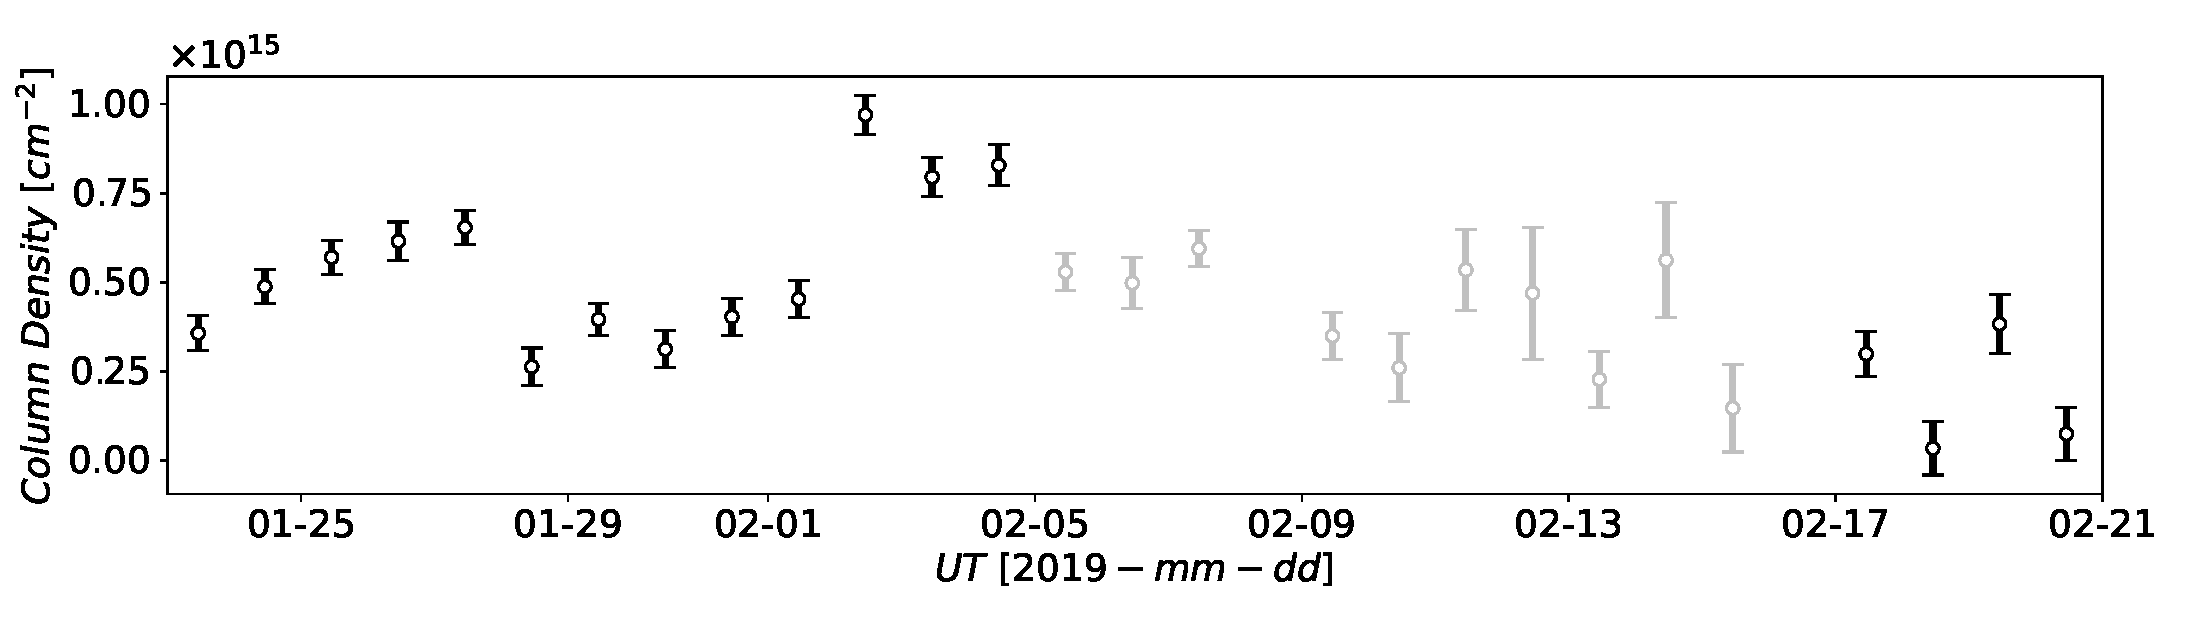
\includegraphics[width=\linewidth]{master_thesis_contents/master_thesis_fig/avg_ColumnDensity_tromsoe.pdf}
    \end{minipage}
    \begin{minipage}{\linewidth}
        \centering
        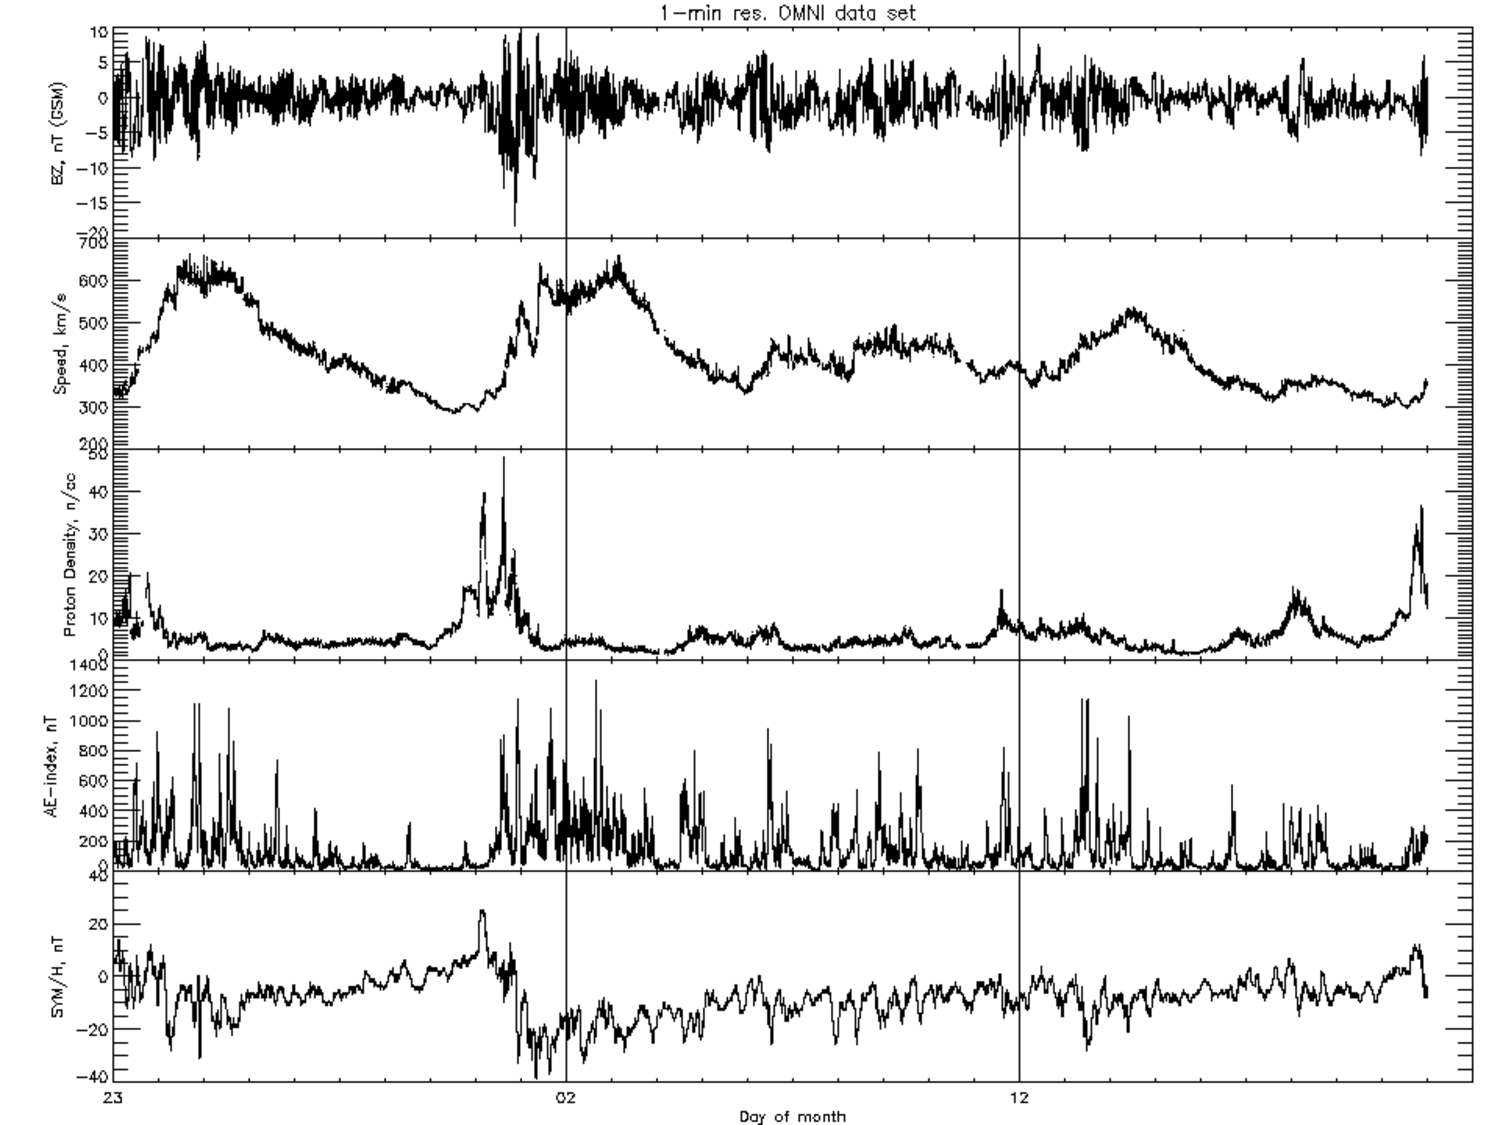
\includegraphics[width=\linewidth]{master_thesis_contents/master_thesis_fig/omni_tromsoe.pdf}
    \end{minipage}
    \caption{トロムソにおける柱密度(1段目。図~\ref{fig:avg_ColumnDensity_tromsoe}と同様)とOMNI Data Set(2段目:地球磁場の南北成分、3段目:太陽風の速さ、4段目:プロトン密度、5段目:AE指数、6段目:SYM/H)との比較}
    \label{fig:omni_mmcd_tromsoe}
\end{figure}

トロムソにおいては、柱密度の増加が確認された2つの期間(2019年1月23日〜2019年1月27日と2019年2月1日〜2019年2月4日)どちらにおいても、地球磁場の南北成分のゆらぎが確認できた。
また、太陽風の速さも大きくなっており、AE指数も何度も激しく値が上昇している。
以上より、SYM/H(もしくは図~\ref{fig:dst_mmcd_tromsoe}のDst指数)の値をみると磁気嵐としての規模に違いはあるが、対象の期間では高速太陽風が吹いており、サブストームが活発にあったことが考えられる。
このことより、高速太陽風が到達した際に磁気圏の活動が活発となり、電子が降り込むことで\ce{NO}の変動に影響を与えたと考えられる。
また、2019年2月1日〜2019年2月4日の期間においては、プロトンの密度も上昇していることが確認された。\par
\begin{figure}[htbp]
    \centering
    \begin{minipage}{\linewidth}
        \centering
        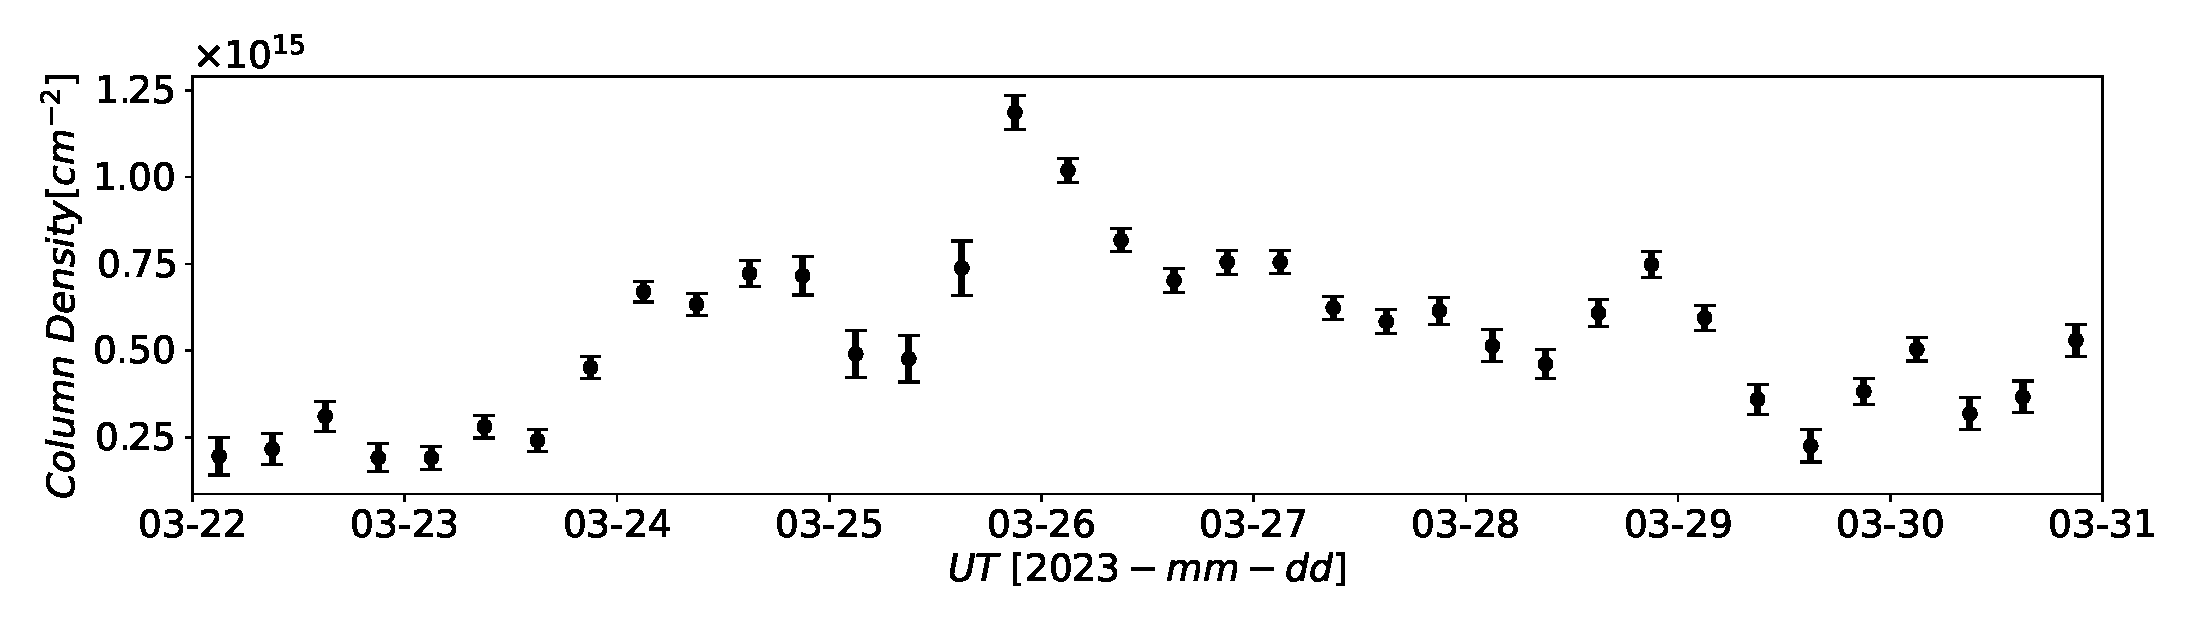
\includegraphics[width=\linewidth]{master_thesis_contents/master_thesis_fig/column_density_spectr6_syowa.pdf}
    \end{minipage}
    \begin{minipage}{0.96\linewidth}
        \centering
        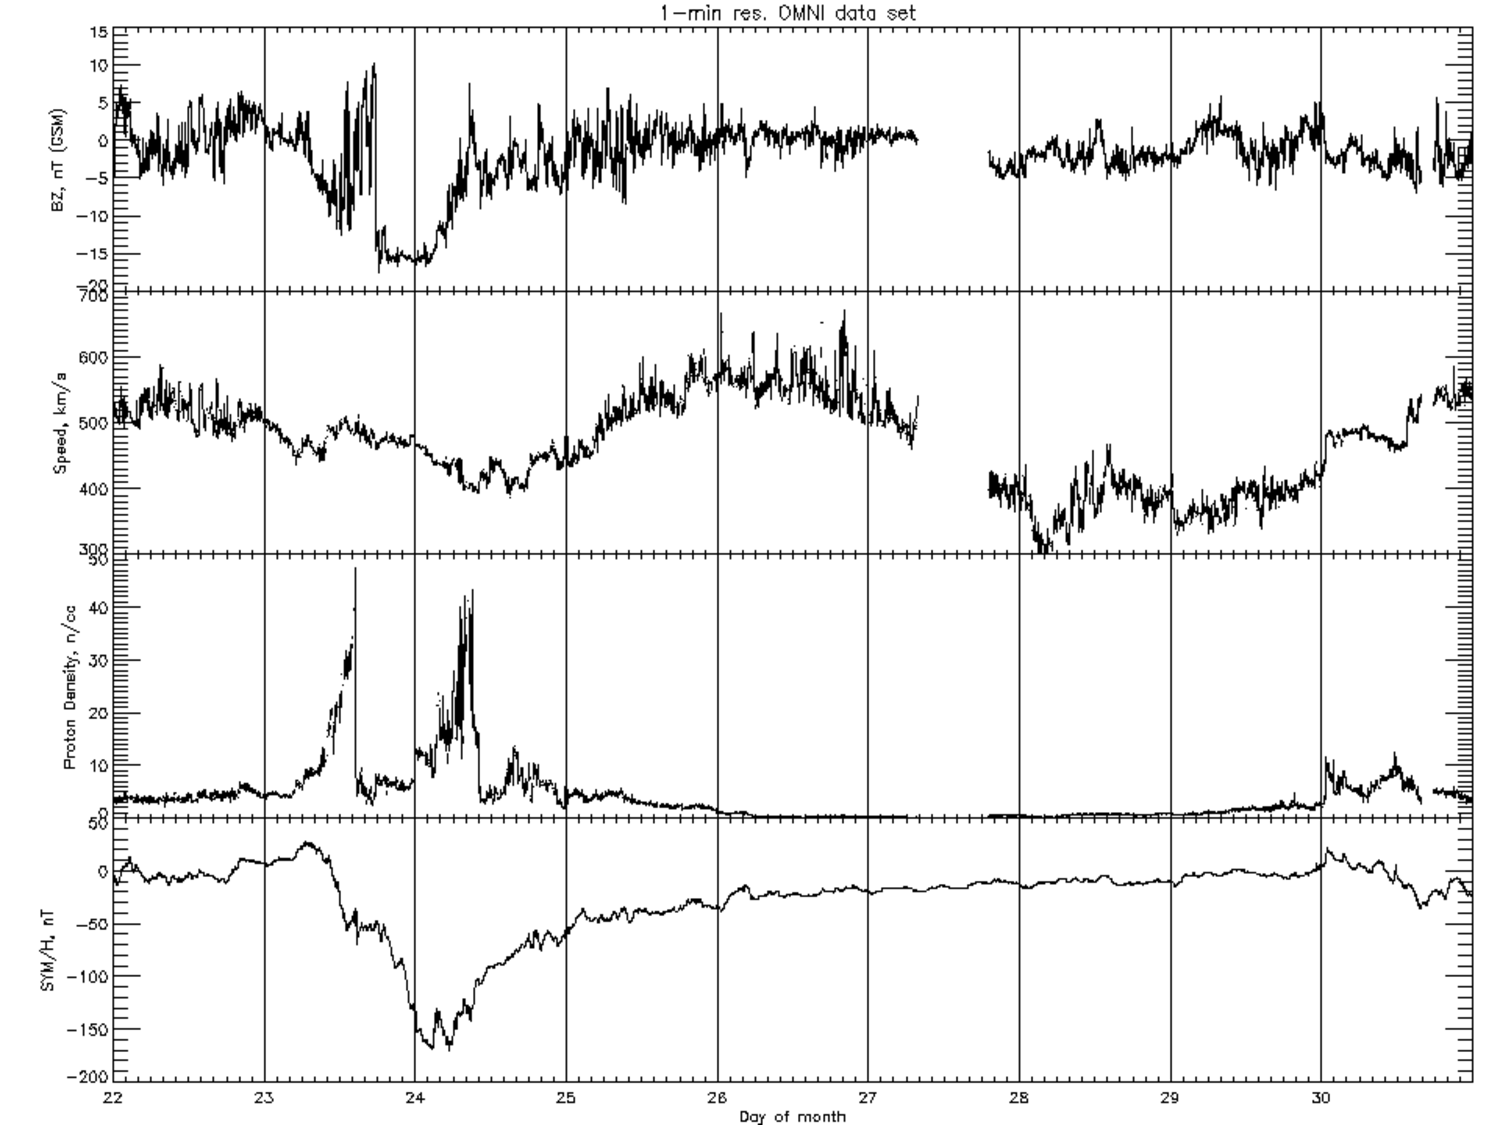
\includegraphics[width=\linewidth]{master_thesis_contents/master_thesis_fig/omni_syowa.pdf}
    \end{minipage}
    \caption{昭和基地における柱密度(1段目。図~\ref{fig:avg_ColumnDensity_tromsoe}と同様)とOMNI Data Set(2段目:地球磁場の南北成分、3段目:太陽風の速さ、4段目:プロトン密度、5段目:SYM/H)との比較}
    \label{fig:omni_mmcd_syowa}
\end{figure}

昭和基地においては、磁気嵐の発生と対応して柱密度が増加した2023年3月23日〜2023年3月24日において地球磁場が南方向を向いており、プロトンの密度も上昇していることが確認された。
しかし、高速太陽風は確認できなかった。
もう1つ柱密度の増加が確認できた2023年3月25日においては、SYM/H(もしくは図~\ref{fig:dst_mmcd_syowa}のDst指数)の値をみると磁気嵐は回復相にあたるが、高速太陽風があることが確認できた。
このことより、磁気圏から回復する期間であっても高速太陽風が到達していると電子の降り込みがあり、\ce{NO}の増加に影響を与えると考えられる。
また、この時期の磁場の振動の中心はわずかに(数nT程度)南向きの状態において高速太陽風が到達しているが、同様な条件で電子フラックスの値が増加することが先行研究~\cite{miyoshi2013high}にて示されている。
